% Перестроение в двумерном случае.
\subsection{Методы перестроения поверхности в двумерном случае}

Consider the geometric problem of rebuilding a surface in two-dimensional space in general form.
Let $n$ cells of the surface grid be given, each of which is represented by a segment of length $l_i$ (that is, the total number of nodes is $n+1$).
The direction of change of the surface of each cell is known (the direction of the normal to the segment), as well as the direction of movement of each node $\overline{g_i}$, $|\overline{g_i}| = 1$.
It coincides with the direction of the sum of the unit normals drawn to the incident cells.
Moreover, for a two-dimensional case, this direction lies on the bisector of the angle formed by two incident cells \cite{Fortin} (Fig.~\ref{fig:grid_normals}).

\begin{figure}[h]
\onelinecaptionstrue
\centering
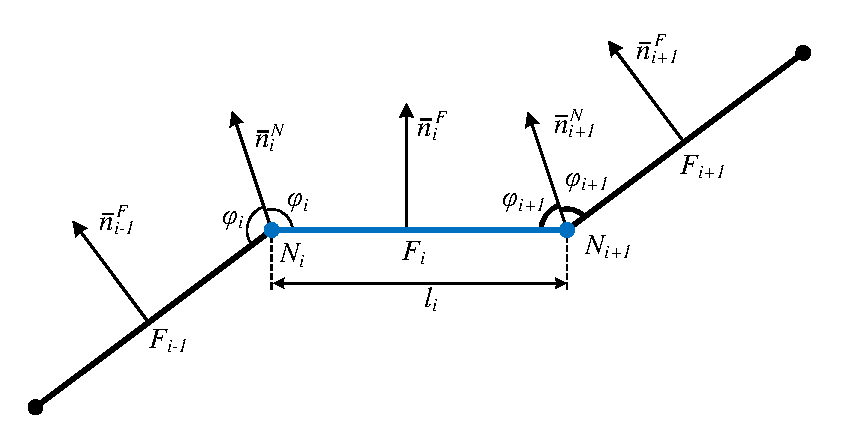
\includegraphics[width=0.8\textwidth]{pics/text_1_remesh_2d/grid_normals.pdf}
\captionstyle{normal}\caption{Surface mesh with designated direction of movement of the nodes.}
\label{fig:grid_normals}
\end{figure}

It is required to find such values of local shifts of grid nodes $h_i$ that the covering area between the old surface and the new surface for each grid cell ($S_i$) differ as small as possible from the required value a $T_i = l_iH_i$.

To solve this problem, first, it's needed to calculate the covering area for each individual cell.

\subsubsection{The task of calculating the covering area when moving nodes of a single cell}

Consider a cell represented on a plane by a segment $AB$ of length $l$.
When moving $A$ and $B$ to the new points $A_1$ and $B_1$ respectively quadrangle $AA_1B_1B$ is formed.
It is required to find its area expressed explicitly through parameters $a = |\overline{AA_1}|$ and $b = |\overline{BB_1}|$ (Fig.~\ref{fig:local}).

\begin{figure}[h]
\onelinecaptionstrue
\centering
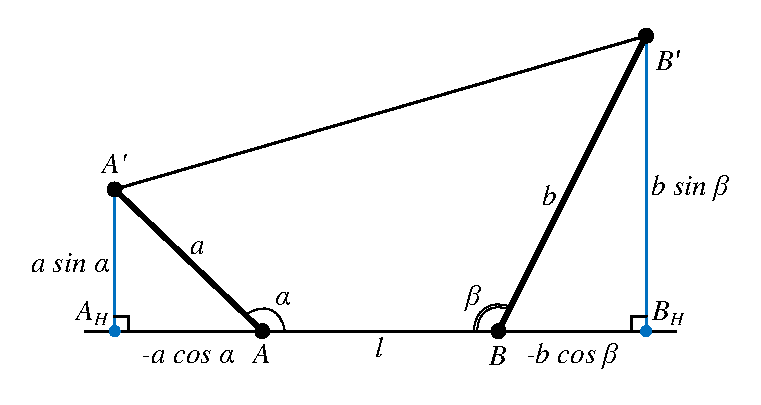
\includegraphics[width=0.8\textwidth]{pics/text_1_remesh_2d/local.pdf}
\captionstyle{normal}\caption{Calculation of the covering area when moving the nodes of the cell.}
\label{fig:local}
\end{figure}

To solve the problem, we drop perpendiculars from the points $A_1$ and $B_1$ to a straight $AB$.
Their projections will be points $A_2$ and $B_2$ respectively.
The required area can be represented as follows:

\begin{equation}
S_{AA_1B_1B} = S_{A_2A_1B_1B_2} - S_{AA_1A_2} - S_{BB_1B_2}
\end{equation}

Denote the angle between the vectors $\overline{AA_1}$ and $\overline{AB}$ as $\alpha$, and the angle between the vectors $\overline{BB_1}$ and $\overline{BA}$ as $\beta$.
Then the required area is calculated explicitly in the following form:

\begin{equation}
S_{AA_1B_1B} = \frac{1}{2}(l - a \cos \alpha - b \cos \beta)(a \sin \alpha + b \sin \beta) + \frac{1}{2}a^2 \sin \alpha \cos \alpha + \frac{1}{2}b^2 \sin \beta \cos \beta
\end{equation}

\begin{equation}
S_{AA_1B_1B} = \frac{1}{2}\big(l(a \sin \alpha + b \sin \beta) - ab \sin(\alpha + \beta)\big)
\end{equation}

\subsubsection{Gradient Descent Solution}

The gradient descent method is one of the simplest optimization method for finding the local minimum of a function.
Provided that at any point of the function it is possible to calculate its gradient, then an iteration sequence is constructed starting from some initial approximation $x_0$.~\cite{Kantorovich}:

\begin{equation}
x^{k+1} = x^k - \gamma _k \nabla f(x_k)
\end{equation}

where $\gamma _k \geq 0$ sets the step length and, respectively, the rate of gradient descend.

The gradient method finds its main application in the task of finding the minimum or maximum of a function.
The direction of the anti-gradient is the direction of the fastest decreasing of the function.
The main problem of the method is to choose the step $\gamma$.
For large values of the step, there is a chance to "jump over" the minimum of the function.
In addition, the method does not guarantee finding a global minimum.

Consider the solution of the problem by the method of gradient descent.
The unknown parameters are the magnitudes of the shifts of the nodes of the grid $h_i$.
Based on the solution of the local problem of determining the covering area, we can define the covering area when a separate cell moves as:

\begin{equation}
S_i = \frac{1}{2}\big(l_i(h_i \sin \alpha_i + h_{i + 1} \sin \beta_i) - h_ih_{i + 1} \sin(\alpha_i + \beta_i)\big) 
\end{equation}

The deviation of the covering area in the cell from the true value will be called the value $\delta_i = S_i - T_i$, and its error is its square $d_i = \delta_i^2$.
The total error when rebuilding the surface is defined as the sum of errors for all cells:

\begin{equation}
D = \sum_{i = 0}^{n - 1}{d_i}
\end{equation}

When finding the optimal solution, it is required to minimize the total error.
To find the gradient, it is required to calculate the partial derivatives of the function $D$ over all unknowns $h_i$.
These derivatives can be written explicitly.

\begin{equation}
\frac{\partial D}{\partial h_i} = \frac{\partial d_{i - 1}}{\partial h_i} + \frac{\partial d_i}{\partial h_i}
\end{equation}

where

\begin{equation}
\begin{cases}
\frac{\partial d_{i - 1}}{\partial h_i} = \delta_{i - 1}(l_{i - 1} \sin \beta_{i - 1} - h_{i - 1} \sin(\alpha_{i - 1} + \beta_{i - 1})) \\
\frac{\partial d_i}{\partial h_i} = \delta_i(l_i \sin \alpha_i - h_{i + 1} \sin(\alpha_i + \beta_i))
\end{cases}
\end{equation}

Also, when implementing the gradient descent method, it is required to monitor the compliance of additional conditions that are imposed on the unknown $h_i$.
For example, an obvious condition is that $h_i \ge 0$ is satisfied, which prevents the grid from moving in a negative direction.
In this work, more stringent conditions $min(H_{i - 1}, H_i) \le h_i \le max(H_{i - 1}, H_i)$ were used, which do not allow the values of the displacement of the grid nodes to go beyond the limits of the displacements of the grid cells incident to them.

\subsubsection{Approximate solution schemes}

Solving the problem of rebuilding the grid using the gradient descent method is too resource-demanding as the grid size increases.
In addition, the quality of the solution is often unsatisfactory, especially when hit in local minima.
Therefore, to solve the problem, methods of approximate solution were proposed, based on approximation of the solution in each cell using primitive geometric shapes.

\subsubsection{Solution by rectangles method}

As a first method, we consider an approximation in which each grid node is shifted by a vector $\frac{1}{2}(H_{i - 1} + H_i)\overline{g_i}$.
This method corresponds to the approximation of the solution in each cell with a rectangle on the sides of $l_i$ and $H_i$, and then averaging, as shown in Fig.~\ref{fig:grid_rectangles}.

\begin{figure}[h]
\onelinecaptionstrue
\centering
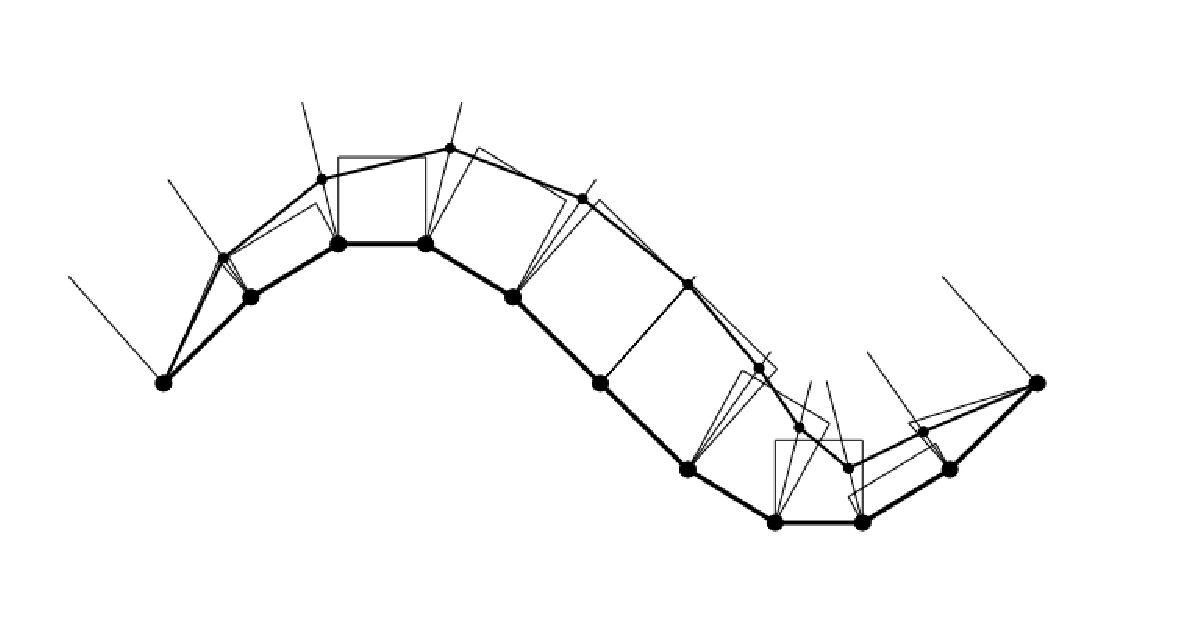
\includegraphics[width=0.8\textwidth]{pics/text_1_remesh_2d/grid_rectangles.pdf}
\captionstyle{normal}\caption{Surface rebuilding using the rectangle method.}
\label{fig:grid_rectangles}
\end{figure}

It is worth noting the possible development of this approach through the use of multilayer approximation, as described in \cite{Bourgault_Cote}, however, this opportunity was not considered in this paper.

\subsubsection{Solution by trapezoid method}

In the trapezoid method, the solution in each cell is approached by a trapezoid with an area of $T_i$, the sides of which lie on the growth directions of two nodes belonging to the considered cell.
After constructing the trapezoid for all grid cells, each internal node has two new potential positions for the shift (formed by the cell on the left and the cell on the right).
Their average value is chosen as the final position. (Fig.~\ref{fig:grid_trapeziums}).

\begin{figure}[h]
\onelinecaptionstrue
\centering
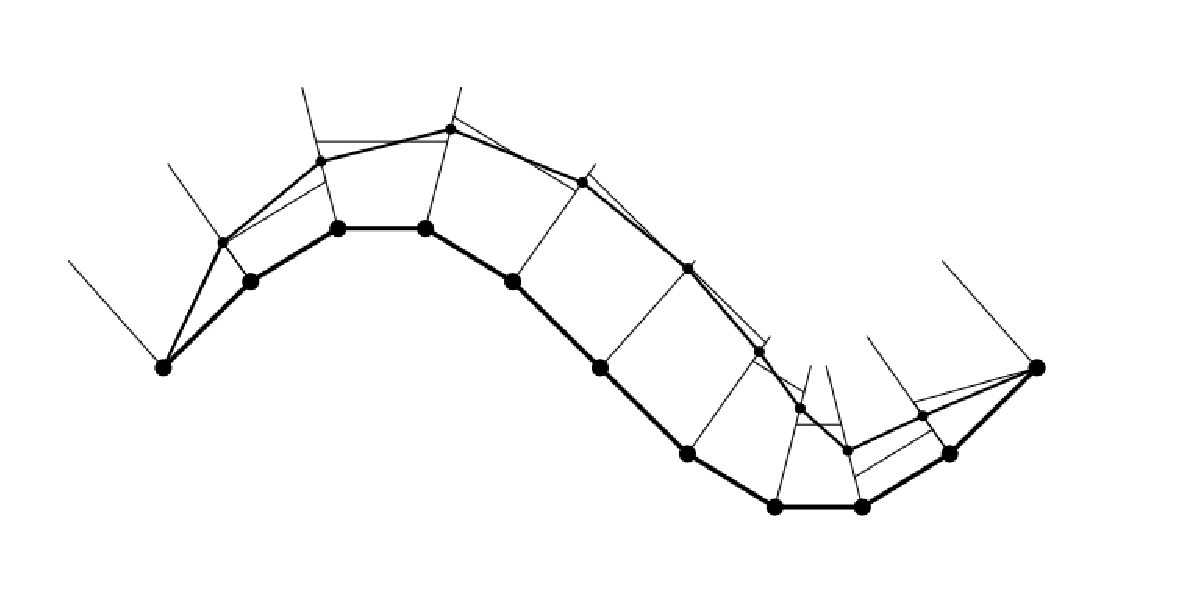
\includegraphics[width=0.8\textwidth]{pics/text_1_remesh_2d/grid_trapeziums.pdf}
\captionstyle{normal}\caption{Surface rebuilding by trapezoid method.}
\label{fig:grid_trapeziums}
\end{figure}

\subsubsection{Comparison of solution accuracy}

To compare the accuracy of the solutions obtained using the methods described, we used a model two-dimensional surface grid represented by a single sinusoid period ($x \in [0, 2 \pi]$).
As a set of cell shifts ($ H_i $), the same shifts equal to half of cell size were used.
With an increase in the number of nodes, both approximate methods demonstrated values $\frac{D}{\sum_i{T_i}}$ tending to zero with minor deviations from each other and from the gradient descent method that was used for verification.
A comparison of the values of $\delta_i$ for all cells for the proposed approximate methods was also carried out.
The results of the comparison on the model grid with the number of nodes $n = 1000$ are shown Fig.~\ref{fig:graphic}.

\begin{figure}[h]
\onelinecaptionstrue
\centering
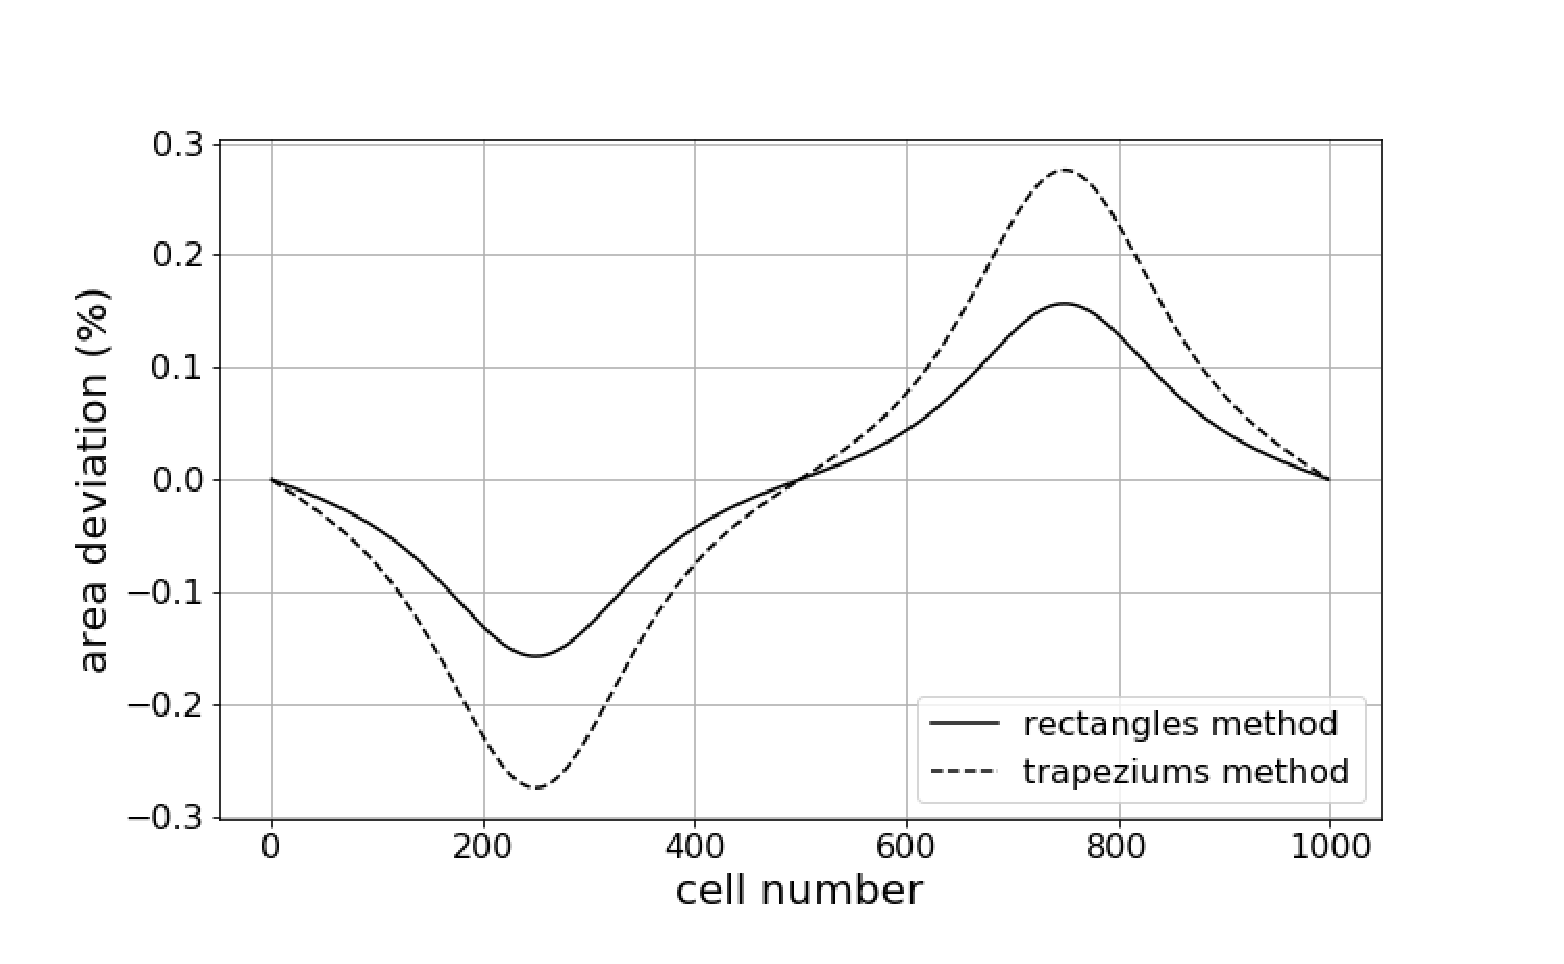
\includegraphics[width=1.0\textwidth]{pics/text_1_remesh_2d/graphic.pdf}
\captionstyle{normal}\caption{Comparison of the accuracy of solutions using the rectangle method and the trapezoid method.}
\label{fig:graphic}
\end{figure}

It can be seen from this graph that the simpler method of rectangles is at the same time more accurate, since it provides smaller deviations from the exact solution on strongly convex and strongly concave sections of the grid.
